\documentclass[aspectratio=169]{beamer}
\usepackage[utf8]{inputenc}
\usepackage[T5]{fontenc}
\usepackage[vietnamese]{babel}
\usepackage{graphicx}
\usepackage{booktabs}
\usepackage{hyperref}
\usepackage{xcolor}
\usepackage{listings}
\usepackage{amsmath}

% Cấu hình giao diện Beamer
\usetheme{Madrid}
\usecolortheme{default}
\setbeamertemplate{navigation symbols}{}
\setbeamertemplate{footline}[frame number]

% Cấu hình màu cho code
\definecolor{codegreen}{rgb}{0,0.6,0}
\definecolor{codegray}{rgb}{0.5,0.5,0.5}
\definecolor{codepurple}{rgb}{0.58,0,0.82}
\definecolor{backcolour}{rgb}{0.95,0.95,0.92}
\lstdefinestyle{mystyle}{
    backgroundcolor=\color{backcolour},   
    commentstyle=\color{codegreen},
    keywordstyle=\color{magenta},
    numberstyle=\tiny\color{codegray},
    stringstyle=\color{codepurple},
    basicstyle=\ttfamily\footnotesize,
    breakatwhitespace=false,         
    breaklines=true,                 
    captionpos=b,                    
    keepspaces=true,                 
    numbers=left,                    
    numbersep=5pt,                  
    showspaces=false,                
    showstringspaces=false,
    showtabs=false,                  
    tabsize=2
}
\lstset{style=mystyle}

\title[TTNT trong Kế toán - Buổi 4]{Trí tuệ Nhân tạo Ứng dụng trong Kế toán}
\subtitle{Buổi 4: Phân khúc Thị trường \& Dự báo Sức khỏe Tài chính}
\author{Giảng viên: [Tên Giảng Viên]}
\institute{Đại học Đông Á}
\date{\today}

\begin{document}

% Slide 1
\begin{frame}
    \titlepage
\end{frame}

% Slide 2
\begin{frame}{Nội dung Bài học}
    \tableofcontents
\end{frame}

% ==========================================
% SECTION 1: Phân khúc Khách hàng & Học không giám sát
% ==========================================
\section{1. Phân khúc Khách hàng \& Học không giám sát}

% Slide 3
\begin{frame}{Chuyển mình sang thuật toán thực chiến}
    \textbf{Từ lý thuyết chung đến ứng dụng thực tiễn:}
    \begin{itemize}
        \item Những buổi trước, chúng ta đã nắm bắt bức tranh toàn cảnh về AI.
        \item \textbf{Buổi 4 đánh dấu bước ngoặt:} Đi sâu vào các thuật toán AI thực chiến (hands-on algorithms).
        \item Không chỉ là lý thuyết, chúng ta sẽ xem xét cách máy móc phân tích các con số để đưa ra quyết định thay con người.
    \end{itemize}
\end{frame}

% Slide 4
\begin{frame}{Hai cột mốc lớn của Bài học}
    \textbf{Chương 5 \& Chương 10:}
    \begin{itemize}
        \item \textbf{Cột mốc 1 (Học không giám sát):} Làm sao để tìm ra đúng tệp khách hàng tiềm năng mà không phải "mò kim đáy bể".
        \item \textbf{Cột mốc 2 (Dự báo sức khỏe tài chính):} Làm cách nào để cứu một doanh nghiệp khỏi bờ vực phá sản bằng các mô hình dự báo tài chính tiên tiến.
    \end{itemize}
\end{frame}

% Slide 5
\begin{frame}{Case Study: Nhà hàng Vegan-Always}
    \begin{block}{Tình huống thực tế tại Phoenix}
        Nhà hàng chay Vegan-Always chuẩn bị khai trương. 
        \begin{itemize}
            \item Câu hỏi đặt ra: Có nên in hàng nghìn voucher (phiếu giảm giá) rồi phát rải thảm khắp thành phố không?
            \item Cách tiếp cận truyền thống: Ai cũng được nhận voucher, hy vọng họ sẽ ghé qua.
        \end{itemize}
    \end{block}
\end{frame}

% Slide 6
\begin{frame}{Vấn đề của "Marketing Đại trà"}
    \textbf{Tại sao "Rải thảm voucher" là một sai lầm?}
    \begin{itemize}
        \item Lãng phí chi phí in ấn và tiếp thị vô ích.
        \item Gửi nhầm thông điệp cho người không có nhu cầu.
        \begin{itemize}
            \item Ví dụ: Một người theo chế độ ăn chỉ toàn thịt (carnivore) sẽ ném voucher món chay vào sọt rác ngay lập tức.
        \end{itemize}
        \item \textit{Bài học:} Cần tìm đúng nhóm người quan tâm đến đồ chay thay vì "đoán mò".
    \end{itemize}
\end{frame}

% Slide 7
\begin{frame}{Khái niệm Phân khúc Thị trường}
    \textbf{Phân khúc Thị trường (Market Segmentation)} là gì?
    \begin{itemize}
        \item Chia một thị trường rộng lớn thành các nhóm khách hàng (phân khúc) có chung các đặc điểm.
        \item Nhắm mục tiêu (Targeting) vào nhóm có khả năng chuyển đổi cao nhất.
        \item Thay vì "tiếp thị đại chúng", ta chuyển sang "tiếp thị tập trung".
    \end{itemize}
\end{frame}

% Slide 8
\begin{frame}{Sự phát triển nhờ Dữ liệu \& AI: Vi phân khúc}
    \textbf{Vi phân khúc (Microsegments) trong thời đại Big Data:}
    \begin{itemize}
        \item Nhờ thu thập dữ liệu hành vi, AI có thể chia thị trường thành những nhóm cực nhỏ.
        \item Không chỉ dừng ở "Phụ nữ 30 tuổi", mà là "Phụ nữ 30 tuổi, thích tập yoga, hay mua đồ online sau 10h tối".
        \item Các ông lớn như Amazon, Netflix đều ứng dụng Vi phân khúc để gợi ý sản phẩm/phim ảnh chính xác đến từng cá nhân.
    \end{itemize}
\end{frame}

% Slide 9
\begin{frame}{Phân khúc Động (Dynamic Segmentation)}
    \textbf{Hành vi khách hàng không đứng im!}
    \begin{itemize}
        \item Khách hàng thay đổi theo thời gian, môi trường, và xu hướng.
        \item AI cho phép cập nhật liên tục phân khúc của một cá nhân theo thời gian thực (Real-time).
    \end{itemize}
\end{frame}

% Slide 10
\begin{frame}{Ví dụ về Phân khúc Động}
    \begin{block}{Sự thay đổi khẩu vị}
        \begin{itemize}
            \item Tháng trước: Khách hàng thường xuyên mua Sô-cô-la đen nguyên chất.
            \item Tháng này: Họ chuyển sang tìm kiếm các loại thực phẩm "Không đường" hoặc "Ít calo".
            \item \textbf{Hệ thống AI:} Lập tức dịch chuyển khách hàng này từ cụm "Tín đồ đồ ngọt" sang cụm "Quan tâm sức khỏe", và bắt đầu quảng cáo bánh ăn kiêng.
        \end{itemize}
    \end{block}
\end{frame}

% Slide 11
\begin{frame}{Khái niệm Học Không giám sát}
    \textbf{Unsupervised Learning là gì?}
    \begin{itemize}
        \item Nghe như "ném bừa dữ liệu vào một hộp đen rồi mặc kệ nó tự tung tự tác"?
        \item Không, "Không giám sát" mang ý nghĩa kỹ thuật: \textbf{Bộ dữ liệu hoàn toàn không có nhãn (Unlabeled Data).}
    \end{itemize}
\end{frame}

% Slide 12
\begin{frame}{Dữ liệu Không nhãn trông như thế nào?}
    \begin{block}{Một đống các con số thô}
        \begin{itemize}
            \item Chúng ta có: Độ tuổi, thu nhập, tần suất mua sắm, giá trị đơn hàng trung bình.
            \item Chúng ta \textbf{KHÔNG CÓ}: Cột phân loại ghi sẵn "Người này thích ăn chay" hay "Người này thích ăn thịt".
            \item Kế toán viên đối diện với hàng vạn dòng dữ liệu mua hàng mà không biết ai thuộc nhóm nào.
        \end{itemize}
    \end{block}
\end{frame}

% Slide 13
\begin{frame}{Khó khăn khi phân tích dữ liệu không nhãn}
    \textbf{Với con người:}
    \begin{itemize}
        \item Việc nhìn chằm chằm vào một bảng Excel có 100,000 dòng và 50 cột dữ liệu để tìm ra các "nhóm khách hàng" là bất khả thi.
        \item Trực giác con người bị giới hạn ở 2-3 chiều không gian.
    \end{itemize}
\end{frame}

% Slide 14
\begin{frame}{Sứ mệnh của Học Không giám sát}
    \textbf{Để máy móc tự làm việc:}
    \begin{itemize}
        \item Thuật toán sẽ tự động "mò mẫm" trong đống dữ liệu hỗn độn.
        \item Sứ mệnh của nó là tìm ra \textbf{cấu trúc ẩn} (hidden structure) bên trong dữ liệu mà không cần con người chỉ bảo trước.
    \end{itemize}
\end{frame}

% Slide 15
\begin{frame}{Phân cụm (Clustering) là gì?}
    \begin{block}{Công cụ cốt lõi của Học không giám sát}
        \textbf{Phân cụm (Clustering):} Là hành động nhóm các điểm dữ liệu lại với nhau dựa trên sự tương đồng của chúng.
        \begin{itemize}
            \item Khách hàng có đặc điểm giống nhau sẽ bị hút về chung một cụm (Cluster).
            \item Một trong những thuật toán nổi tiếng nhất để làm việc này là \textbf{k-Means}.
        \end{itemize}
    \end{block}
\end{frame}

% Slide 16
\begin{frame}{Chuyển ý: Đi sâu vào Thuật toán}
    \begin{center}
        \Large Làm thế nào mà thuật toán k-Means biết hai khách hàng có "hành vi giống nhau" để xếp chung vào một cụm?\\
        \vspace{1cm}
        \textit{Chúng ta cùng tìm hiểu phần tiếp theo!}
    \end{center}
\end{frame}

% ==========================================
% SECTION 2: Thuật toán k-Means, k-Medoid & Hệ số Silhouette
% ==========================================
\section{2. Thuật toán k-Means, k-Medoid \& Hệ số Silhouette}

% Slide 17
\begin{frame}{Thuật toán k-Means: Cơ chế Đo khoảng cách}
    \textbf{Khoảng cách (Distance) trong toán học:}
    \begin{itemize}
        \item Thuật toán k-Means sử dụng "khoảng cách" để đo lường sự tương đồng giữa các khách hàng.
        \item Hãy tưởng tượng mỗi người khách là một điểm trên trục tọa độ.
    \end{itemize}
\end{frame}

% Slide 18
\begin{frame}{Mối quan hệ: Khoảng cách \& Sự tương đồng}
    \textbf{Khoảng cách ngắn = Hành vi giống nhau}
    \begin{itemize}
        \item Điểm A (Khách 1) và Điểm B (Khách 2) nằm sát nhau.
        \item Đoạn thẳng nối hai điểm đó càng ngắn, tức là hành vi tiêu dùng (ví dụ số tiền chi, số lần mua) của hai người đó càng giống nhau.
        \item K-Means luôn cố gắng gom những người "đứng gần nhau" vào cùng một cụm.
    \end{itemize}
\end{frame}

% Slide 19
\begin{frame}{Ví dụ trực quan: Bữa tiệc khổng lồ \& lộn xộn}
    \textbf{Bước 1: Chọn số lượng bàn (k)}
    \begin{itemize}
        \item Hãy tưởng tượng bạn đang tổ chức một bữa tiệc khổng lồ.
        \item Ban đầu, bạn chọn một số lượng bàn tiệc nhất định, gọi là $k$.
        \item Bạn đặt ngẫu nhiên $k$ chiếc bàn giữa căn phòng lộn xộn. (Các chiếc bàn này đại diện cho các \textbf{tâm cụm - Centroid}).
    \end{itemize}
\end{frame}

% Slide 20
\begin{frame}{Ví dụ trực quan: Bữa tiệc khổng lồ \& lộn xộn (Tiếp)}
    \textbf{Bước 2: Gán điểm (Assign)}
    \begin{itemize}
        \item Các khách mời (đại diện cho Dữ liệu khách hàng) tiến vào phòng.
        \item Họ sẽ tự động nhìn quanh và chạy đến chiếc bàn nào \textbf{gần họ nhất}.
        \item Lúc này, khách đã "bu quanh" các bàn.
    \end{itemize}
\end{frame}

% Slide 21
\begin{frame}{Ví dụ trực quan: Bữa tiệc khổng lồ \& lộn xộn (Tiếp)}
    \textbf{Bước 3: Dời tâm (Update)}
    \begin{itemize}
        \item Bạn nhận ra: Chiếc bàn lúc này bị lệch, nó không còn nằm ở chính giữa nhóm khách đang bu quanh nó nữa.
        \item Thế là bạn hì hục khiêng chiếc bàn dời vào đúng \textbf{trung tâm (trọng tâm)} của nhóm khách đó.
    \end{itemize}
\end{frame}

% Slide 22
\begin{frame}{Ví dụ trực quan: Bữa tiệc khổng lồ \& lộn xộn (Tiếp)}
    \textbf{Bước 4: Sự thay đổi \& Hội tụ}
    \begin{itemize}
        \item Khi bạn dời bàn, một số người ở rìa bất ngờ thấy: \textit{"Ô, cái bàn nhóm khác giờ lại gần mình hơn cái bàn hiện tại!"}
        \item Họ liền chạy sang nhóm khác.
        \item Bạn lại phải tiếp tục dời bàn.
        \item \textbf{Điểm Hội tụ:} Lặp đi lặp lại quy trình này cho đến khi không còn khách nào muốn chuyển bàn nữa (Trạng thái ổn định nhất).
    \end{itemize}
\end{frame}

% Slide 23
\begin{frame}{Cấu trúc Lặp của k-Means (Tóm tắt)}
    \begin{block}{Quy trình thuật toán (Vòng lặp tối ưu)}
        \begin{enumerate}
            \item \textbf{Khởi tạo:} Chọn ngẫu nhiên $k$ tâm cụm ban đầu.
            \item \textbf{Bước Gán (Assignment):} Gán mỗi điểm dữ liệu vào tâm cụm gần nhất.
            \item \textbf{Bước Cập nhật (Update):} Tính toán lại vị trí tâm cụm mới dựa trên trung bình cộng của các điểm trong cụm.
            \item \textbf{Kiểm tra:} Lặp lại Bước 2 và Bước 3 cho đến khi vị trí các tâm cụm không thay đổi.
        \end{enumerate}
    \end{block}
\end{frame}

% Slide 24
\begin{frame}{Hạn chế của k-Means}
    \textbf{Nhược điểm cực lớn: Nhạy cảm với Điểm ngoại lai (Outliers)}
    \begin{itemize}
        \item Tâm cụm của k-Means được tính bằng \textbf{Trung bình cộng (Mean)}.
        \item Nếu trong bữa tiệc có một "vị khách khổng lồ" đứng tuốt ngoài góc phòng, phép tính trung bình sẽ kéo lê chiếc bàn (tâm cụm) về phía góc đó một cách vô lý.
    \end{itemize}
\end{frame}

% Slide 25
\begin{frame}{Tại sao Dữ liệu Kế toán lại nhiều Outliers?}
    \begin{itemize}
        \item Trong tài chính kế toán, dữ liệu thường bị lệch (skewed).
        \item Đa số khách hàng chi 1 triệu đồng/tháng, nhưng thỉnh thoảng có vài khách sỉ chi tới 500 triệu đồng/tháng.
        \item Các khách hàng "đột biến" này sẽ phá hỏng mô hình k-Means thông thường.
    \end{itemize}
\end{frame}

% Slide 26
\begin{frame}{Giải pháp: Thuật toán k-Medoid}
    \textbf{Chống nhiễu (Robust) tốt hơn k-Means!}
    \begin{itemize}
        \item \textbf{Khác biệt lõi:} Thay vì dùng giá trị "Trung bình cộng" (vô hình) làm tâm, k-Medoid sử dụng một \textbf{điểm dữ liệu thực tế} (Medoid) để làm tâm.
        \item Giống như việc bạn chọn ra một vị khách tiêu biểu nhất trong nhóm làm "trưởng bàn", và lấy vị trí của người đó làm tâm cụm.
        \item Trưởng bàn là người thực, nên không bị kéo lê bởi một vài cá nhân cực đoan bên ngoài.
    \end{itemize}
\end{frame}

% Slide 27
\begin{frame}{Làm sao biết $k$ bằng bao nhiêu?}
    \textbf{Một câu hỏi kinh điển trong Machine Learning!}
    \begin{itemize}
        \item Cả k-Means và k-Medoid đều \textbf{không tự biết} $k$ bằng bao nhiêu.
        \item Bạn phải nói cho nó biết bạn muốn chia thành 2, 3, hay 5 nhóm.
        \item Nếu đoán mò số $k$, kết quả có thể rất tồi tệ. Ta cần một công cụ chấm điểm để tìm $k$ tối ưu.
    \end{itemize}
\end{frame}

% Slide 28
\begin{frame}{Hệ số Silhouette (Silhouette Width)}
    \textbf{Công cụ đo lường chất lượng cụm}
    \begin{itemize}
        \item Silhouette chấm điểm dựa trên mức độ hợp lý của việc chia nhóm.
        \item Dao động từ \textbf{-1 đến 1}.
        \item Nếu điểm số càng gần 1, chứng tỏ các cụm rất gắn kết bên trong và tách biệt rõ ràng với bên ngoài $\rightarrow$ \textbf{Lý tưởng!}
    \end{itemize}
\end{frame}

% Slide 29
\begin{frame}{Hai tiêu chí cốt lõi của Silhouette}
    \begin{block}{Cách tính điểm Silhouette}
        \begin{enumerate}
            \item \textbf{Độ gắn kết (Cohesion):} Các điểm dữ liệu trong cùng một cụm có nằm sát nhau không? (Càng sát càng tốt).
            \item \textbf{Độ tách biệt (Separation):} Hai cụm khác nhau có nằm xa nhau không? (Càng xa càng tốt để tránh nhầm lẫn).
        \end{enumerate}
    \end{block}
\end{frame}

% Slide 30
\begin{frame}{Ứng dụng Kế toán: Phân khúc để tối ưu lợi nhuận}
    \textbf{Biến phân tích:} Số tiền chi tiêu \& Thời gian gắn bó.
    \begin{itemize}
        \item Thuật toán chỉ ra 2 cụm hoàn toàn trái ngược:
        \item \textbf{Cụm 1:} Khách gắn bó rất lâu (chậm rời bỏ) nhưng tiêu rất ít tiền.
        \item \textbf{Cụm 2:} Khách vừa gắn bó lâu, lại vừa chi rất nhiều tiền.
        \item \textbf{Hành động Kế toán Quản trị:} Lập tức dồn lực Marketing \& Chăm sóc khách hàng vào Cụm 2 để tối ưu hóa ROI (Tỷ suất hoàn vốn).
    \end{itemize}
\end{frame}

% Slide 31
\begin{frame}[fragile]{Thực hành R: Code k-Means cơ bản}
    \begin{lstlisting}[language=R]
# Goi cac thu vien can thiet
library(cluster)
library(factoextra)

# Chuan hoa du lieu ve don vi Z-score (Quan trong)
df_scaled <- scale(df, center = TRUE, scale = TRUE)

# Chay thuat toan k-Means voi k = 3
# nstart = 25 nghia la thu 25 lan dat ban ngau nhien 
# de tim ket qua hoi tu tot nhat
k_means <- kmeans(df_scaled, centers = 3, nstart = 25)

# In thu ket qua
print(k_means$centers)
    \end{lstlisting}
\end{frame}

% Slide 32
\begin{frame}{Kết quả Trực quan: Biểu đồ k-Means}
    \begin{columns}
        \column{0.5\textwidth}
        \textbf{Phân tích Hình 5.4:}
        \begin{itemize}
            \item Dữ liệu đã được gán vào 3 cụm (clusters) riêng biệt.
            \item Hàm \texttt{fviz\_cluster()} trong package \texttt{factoextra} giúp vẽ vùng bao quanh các cụm.
            \item Rất trực quan để trình bày trước Ban Giám đốc.
        \end{itemize}
        
        \column{0.5\textwidth}
        \begin{figure}
            \centering
            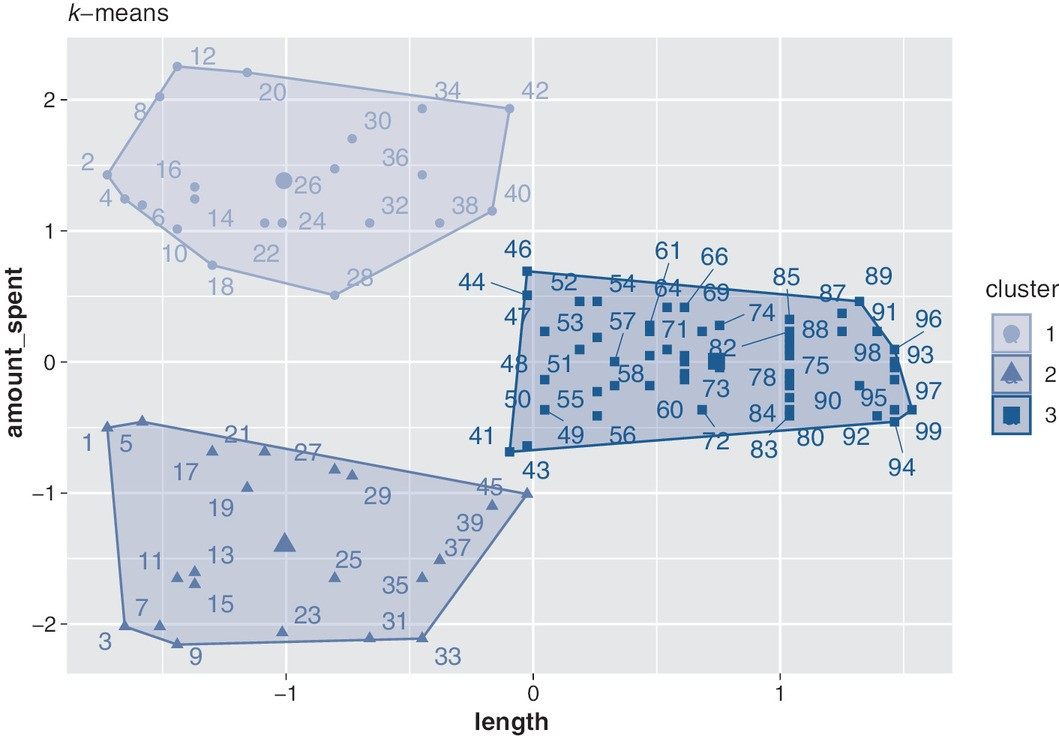
\includegraphics[width=0.9\textwidth]{../../Figures/Buoi_04A/Figure 5.4 k-Means Segmentation Plot.jpeg}
            \caption{k-Means Segmentation Plot}
        \end{figure}
    \end{columns}
\end{frame}

% ==========================================
% SECTION 3: Dự báo Phá sản, Đa cộng tuyến & Hồi quy LASSO
% ==========================================
\section{3. Dự báo Phá sản, Đa cộng tuyến \& Hồi quy LASSO}

% Slide 33
\begin{frame}{Bảo vệ Sinh mệnh Doanh nghiệp}
    \textbf{Từ tìm kiếm khách hàng sang bảo vệ dòng tiền:}
    \begin{itemize}
        \item Bán được nhiều hàng để tăng doanh thu sẽ vô nghĩa nếu bản thân doanh nghiệp đang rỉ máu tài chính từ bên trong.
        \item Bán nhiều hàng $\neq$ Không thể phá sản.
        \item Chúng ta chuyển sang bài toán: Đánh giá sức khỏe tài chính và Dự báo rủi ro vỡ nợ.
    \end{itemize}
\end{frame}

% Slide 34
\begin{frame}{Dự báo Phá sản: Góc nhìn Người cho vay}
    \begin{block}{Tình huống: Ngân hàng UltraBank}
        Khi đánh giá hồ sơ vay vốn của một doanh nghiệp, UltraBank phải tính toán xác suất doanh nghiệp đó sẽ phá sản trong 1-2 năm tới.
    \end{block}
    \textbf{Công cụ truyền thống:} Tính toán các Tỷ số tài chính (Financial Ratios).
\end{frame}

% Slide 35
\begin{frame}{Các Chỉ số Tài chính phổ biến}
    Sinh viên Kế toán nào cũng phải học những chỉ số này:
    \begin{itemize}
        \item Tỷ số Nợ trên Vốn chủ sở hữu (Debt-to-Equity).
        \item Tỷ số thanh toán hiện hành (Current Ratio).
        \item Tỷ số thanh toán nhanh (Quick Ratio).
        \item Biên lợi nhuận ròng (Net Profit Margin).
    \end{itemize}
\end{frame}

% Slide 36
\begin{frame}{Vấn đề: Sử dụng quá nhiều chỉ số}
    \textbf{Nhiều chưa chắc đã tốt!}
    \begin{itemize}
        \item Trong kỷ nguyên Big Data, chúng ta có thể tính ra hàng trăm tỷ số tài chính khác nhau.
        \item Nhét tất cả các tỷ số này vào một mô hình Hồi quy truyền thống (OLS) sẽ gây ra một "căn bệnh" chí mạng.
        \item Đó là hiện tượng: \textbf{Đa cộng tuyến (Multicollinearity).}
    \end{itemize}
\end{frame}

% Slide 37
\begin{frame}{Hiện tượng Đa cộng tuyến là gì?}
    \textbf{Định nghĩa Thống kê:}
    \begin{itemize}
        \item Đa cộng tuyến xảy ra khi các biến độc lập (predictors) trong mô hình có sự tương quan cực kỳ chặt chẽ với nhau.
        \item Thông tin bị lặp đi lặp lại dư thừa.
    \end{itemize}
\end{frame}

% Slide 38
\begin{frame}{Ví dụ Trực quan: Lái xe với 5 chiếc GPS}
    \begin{exampleblock}{Đa cộng tuyến qua hình ảnh 5 cái GPS}
        \begin{itemize}
            \item Tưởng tượng bạn đang lái xe, và bạn bật \textbf{5 chiếc máy GPS} cùng lúc để chỉ đường.
            \item Các máy này chỉ đường gần giống hệt nhau, nhưng thỉnh thoảng cái này kêu "Rẽ phải", cái kia vừa kêu xong lại có độ trễ.
            \item Chúng \textbf{gào thét tạo ra sự nhiễu loạn}. 
            \item Thay vì giúp bạn đến đích an toàn, mớ âm thanh hỗn độn đó làm bạn hoảng loạn và đâm xe!
        \end{itemize}
    \end{exampleblock}
\end{frame}

% Slide 39
\begin{frame}{Hậu quả với Hồi quy Cổ điển (OLS)}
    \textbf{Mô hình OLS (Bình phương Tối thiểu) thất bại thảm hại:}
    \begin{itemize}
        \item OLS có một giả định cốt lõi: Các biến độc lập \textbf{KHÔNG ĐƯỢC} tương quan mạnh với nhau.
        \item Khi 5 chiếc GPS (các biến đa cộng tuyến) cùng gào thét, OLS không biết nên nghe theo biến nào.
    \end{itemize}
\end{frame}

% Slide 40
\begin{frame}{Tại sao OLS thất bại trước Đa cộng tuyến?}
    \textbf{Về mặt toán học:}
    \begin{itemize}
        \item Sai số chuẩn (Standard Error) của các hệ số sẽ \textbf{tăng vọt}.
        \item Gây ra \textbf{Sai lầm Loại II}: Mô hình bác bỏ những cảnh báo nguy hiểm thực sự.
        \item Giống như chuông báo cháy đang kêu, nhưng Đa cộng tuyến đã bóp nghẹt âm thanh đó đi. Hậu quả là Ngân hàng cho một công ty sắp sụp đổ vay tiền!
    \end{itemize}
\end{frame}

% Slide 41
\begin{frame}{Phát hiện Đa cộng tuyến (Correlation Plot)}
    \begin{columns}
        \column{0.5\textwidth}
        \textbf{Phân tích Hình 10.2:}
        \begin{itemize}
            \item Dùng Biểu đồ Tương quan (Correlation Plot) để khám bệnh.
            \item Nếu thấy tỷ lệ tương quan $> 0.9$ (màu xanh/đỏ rất đậm), Đa cộng tuyến đang xảy ra.
            \item Hệ số VIF (Variance Inflation Factor) có khi lên tới \textbf{600} (Mức báo động đỏ).
        \end{itemize}
        
        \column{0.5\textwidth}
        \begin{figure}
            \centering
            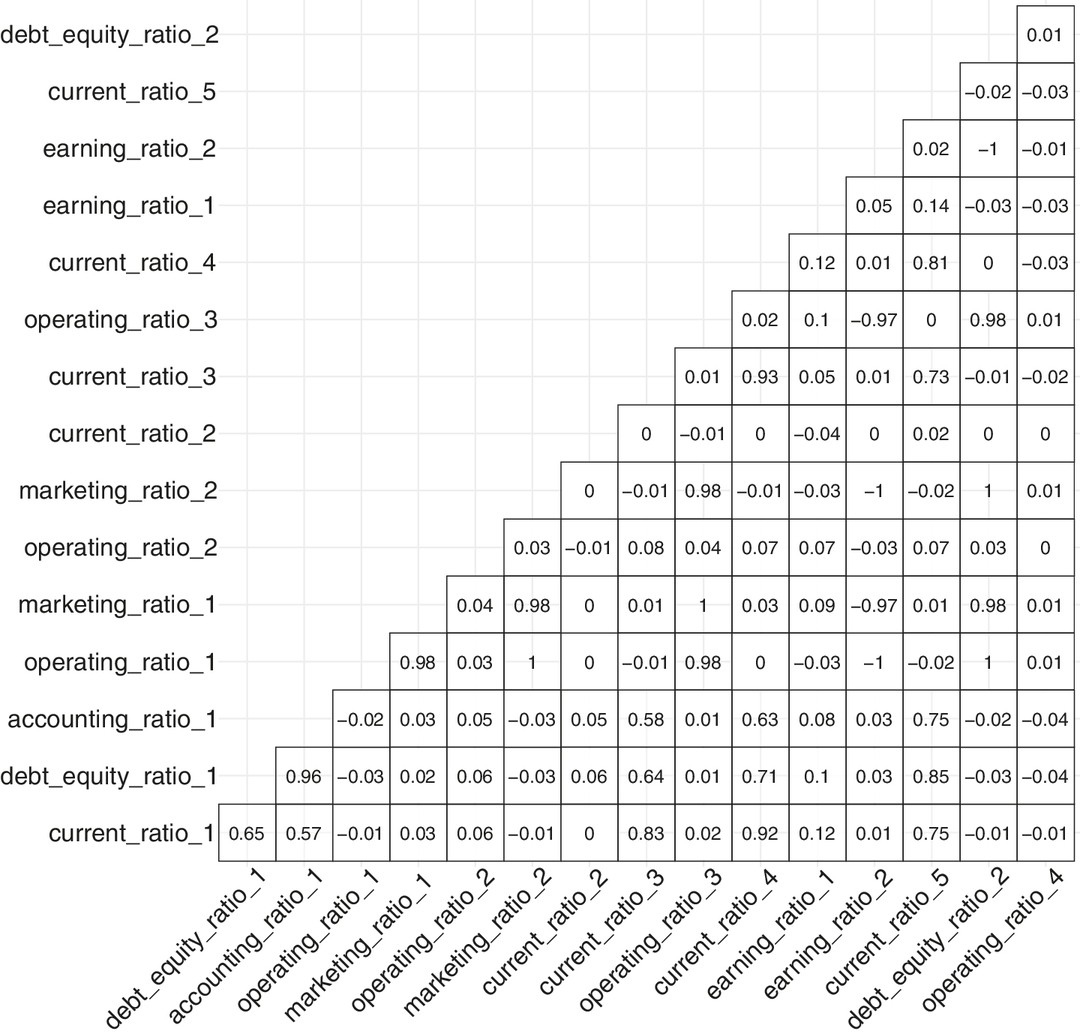
\includegraphics[width=0.9\textwidth]{../../Figures/Buoi_04B/Figure 10.2 Correlation Plot.jpeg}
            \caption{Ma trận tương quan}
        \end{figure}
    \end{columns}
\end{frame}

% Slide 42
\begin{frame}{Giải pháp AI: Rời bỏ OLS, chuyển sang Hồi quy có phạt}
    \textbf{UltraBank cần một lối thoát!}
    \begin{itemize}
        \item Chuyển sang sử dụng thuật toán \textbf{Penalized Regression (Hồi quy có phạt)}.
        \item Thuật toán tiêu biểu nhất: \textbf{LASSO (Least Absolute Shrinkage and Selection Operator)}.
    \end{itemize}
\end{frame}

% Slide 43
\begin{frame}{Sự trừng phạt dữ liệu của LASSO}
    \textbf{Nghe như máy móc đang "đi trừng phạt" dữ liệu?}
    \begin{itemize}
        \item Đúng vậy! LASSO thêm một Thuật ngữ phạt, ký hiệu là $\lambda$ (Lambda) vào phương trình.
        \item Khi $\lambda$ tăng lên, LASSO sẽ trừng phạt các hệ số ($\beta$) của những chỉ số tài chính không quan trọng (những chiếc GPS gây nhiễu).
    \end{itemize}
\end{frame}

% Slide 44
\begin{frame}{Cơ chế Trừng phạt: Ép về 0}
    \begin{block}{Sức mạnh lớn nhất của LASSO}
        Thuật toán này ép các hệ số gây nhiễu teo nhỏ lại, và cuối cùng \textbf{ép về đúng bằng số 0}.
        \begin{itemize}
            \item Hệ số = 0 nghĩa là tỷ số tài chính đó đã bị loại bỏ hoàn toàn khỏi mô hình dự báo!
        \end{itemize}
    \end{block}
\end{frame}

% Slide 45
\begin{frame}{Tự động Lựa chọn Biến (Variable Selection)}
    \textbf{Tối ưu hóa đáng kinh ngạc:}
    \begin{itemize}
        \item UltraBank đo lường 16 tỷ số tài chính khác nhau.
        \item Khủng hoảng Đa cộng tuyến (VIF > 600).
        \item LASSO tự động vung gươm, chém 4 tỷ số nhiễu ép về 0.
        \item Chỉ giữ lại \textbf{12 tỷ số thực sự cốt lõi} để dự báo. Kế toán viên không cần phải tự ngồi đoán xem biến nào quan trọng nữa!
    \end{itemize}
\end{frame}

% Slide 46
\begin{frame}{Đánh giá Mô hình: Đường cong AUC ROC}
    \textbf{Làm sao Ngân hàng dám tin tưởng thuật toán LASSO để giao tiền?}
    \begin{itemize}
        \item Ta dùng công cụ đo lường gọi là Đường cong ROC.
        \item \textbf{Trục Y:} Tỷ lệ \textit{True Positive} (Đoán đúng công ty phá sản).
        \item \textbf{Trục X:} Tỷ lệ \textit{False Positive} (Báo động nhầm - Công ty khỏe mà bảo phá sản).
    \end{itemize}
\end{frame}

% Slide 47
\begin{frame}{Ý nghĩa của Điểm số AUC (Area Under the Curve)}
    \textbf{Cách chấm điểm ROC AUC:}
    \begin{itemize}
        \item \textbf{AUC = 0.5:} Mô hình vô dụng. Nó dự báo bừa bãi không khác gì nhắm mắt tung đồng xu.
        \item \textbf{AUC = 1.0:} Hoàn hảo tuyệt đối.
        \item Vậy trong thực tế tài chính, điểm số AUC bao nhiêu là đủ tốt để ứng dụng?
    \end{itemize}
\end{frame}

% Slide 48
\begin{frame}{Kết quả Đánh giá Mô hình LASSO}
    \begin{columns}
        \column{0.5\textwidth}
        \textbf{Phân tích Hình 10.4:}
        \begin{itemize}
            \item Mô hình LASSO đạt \textbf{AUC $\approx$ 0.8}.
            \item Đây là một con số rất tốt và ấn tượng!
            \item UltraBank hoàn toàn tự tin nhập số liệu doanh nghiệp mới vào hệ thống.
            \item Mô hình xuất ra \textbf{0 (Từ chối vay)} hoặc \textbf{1 (An toàn, duyệt khoản vay)}.
        \end{itemize}
        
        \column{0.5\textwidth}
        \begin{figure}
            \centering
            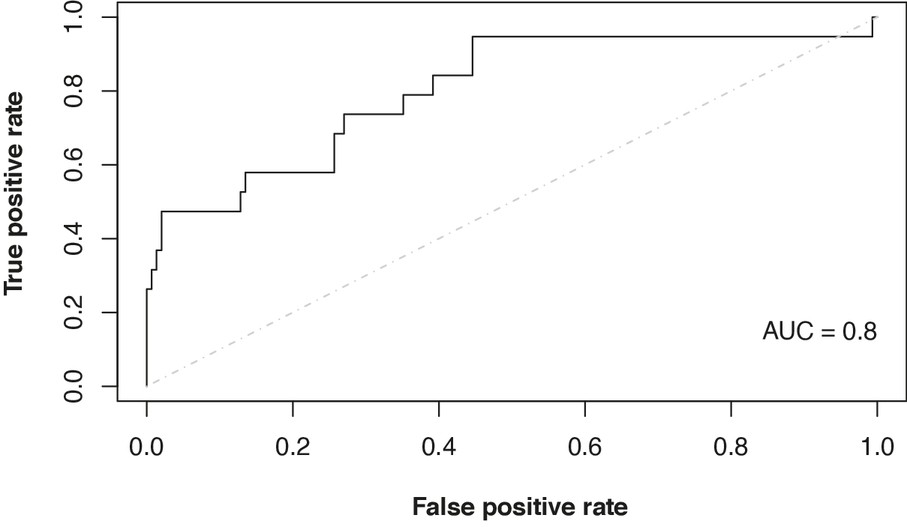
\includegraphics[width=0.9\textwidth]{../../Figures/Buoi_04B/Figure 10.4 AUC ROC Curve.jpeg}
            \caption{Đường cong AUC ROC}
        \end{figure}
    \end{columns}
\end{frame}

% Slide 49
\begin{frame}{Tổng kết: Sự va chạm giữa Con người \& Máy móc}
    \textbf{Nhìn lại Chặng đường Buổi 4:}
    \begin{itemize}
        \item Dùng k-Means để gom nhóm dữ liệu hỗn loạn, tìm ra \textit{Khách hàng Vàng}.
        \item Dùng LASSO để vượt qua đám sương mù Đa cộng tuyến, tìm ra \textit{Chỉ số sống còn}.
        \item Kế toán vốn từ xưa đến nay dựa trên nguyên tắc và phán đoán của con người. Nhưng thuật toán lại có thể ép bỏ những chỉ số mà "sách giáo khoa kinh điển coi là quan trọng"!
    \end{itemize}
\end{frame}

% Slide 50
\begin{frame}{Câu hỏi mở: Trực giác vs. Thuật toán}
    \begin{block}{Một câu hỏi hóc búa cho Kế toán tương lai}
        Nếu dự báo của một hệ thống AI \textbf{mâu thuẫn hoàn toàn} với trực giác của một Kế toán trưởng có 20 năm kinh nghiệm... \\
        \textbf{Chúng ta nên nghe ai?}
    \end{block}
\end{frame}

% Slide 51
\begin{frame}{Tương lai của ngành Kế toán - Tài chính}
    \begin{itemize}
        \item Tương lai không phải là \textbf{phục tùng AI} một cách mù quáng.
        \item Kế toán viên phải học cách \textbf{diễn dịch, kiểm soát và tranh luận} với các kết quả máy móc đưa ra.
        \item Máy móc có thể tính toán nhanh hơn, nhưng Quyết định cuối cùng và Đạo đức nghề nghiệp thuộc về con người!
    \end{itemize}
\end{frame}

% Slide 52
\begin{frame}
    \centering
    \Huge \textbf{Cảm ơn các bạn đã lắng nghe!}
    
    \vspace{0.5cm}
    \Large Hỏi \& Đáp
\end{frame}

\end{document}
